\documentclass[10pt,letterpaper]{book}
\usepackage[utf8]{inputenc}
\usepackage[T1]{fontenc}
\usepackage{lmodern}
\usepackage{amsmath}
\usepackage{amsfonts}
\usepackage{amssymb}
\usepackage{color}
\usepackage{listings}
\usepackage{graphicx}
\usepackage{longtable}

\graphicspath{ {images/} }

\newcommand{\todo}[1]{\textcolor{red}{#1}}
\newcommand{\comment}[1]{\textcolor{red}{#1}}
\newcommand{\filename}[1]{\textit{#1}}

\author{Eric Moyer}
\title{Skip-gram Extraction of Personality Components from News Corpora}
\begin{document}
\frontmatter
\maketitle

\chapter{Abstract}
Vector-based lexical semantics is a powerful technique that still has many undiscovered applications. In this thesis I apply a skip-gram lexical-semantic model newly developed by Mikolov et. al. to the lexical hypothesis in personality psychology.

\mainmatter
\chapter{Introduction}

When the ghost of Jacob Marley confronted Ebenezer Scrooge in ``A Christmas Carol,'' Scrooge tried to justify his former partner by saying ``But you were always a good man of business, Jacob!'' Marley responded with the anguished cry, ``Business! Mankind was my business. \ldots The dealings of my trade were but a drop of water in the comprehensive ocean of my business!'' To those who wish that their dealings this life would benefit not only the easily modeled \textit{homo economicus} but also the rest of our irrational species, it is necessary to understand people. This is the domain of the humanities and social sciences. Among its students are economists, political scientists, linguists, historians, sociologists, psychologists, and anthropologists. Of these, the ones who attempt to understand the mental functions of people are the psychologists.

Finding the invariants in any particular field has been an incredibly successful method of study through the ages. The mental invariants that characterize a person over periods of time are that person's personality. Since the 1980's, many personality psychologists have begun using trait models derived from factor analysis of people's usage of language in describing others. The most famous of these is the Five Factor Model measured by McCrae and Costa's NEO inventory. It measures personality along the five dimensions of Openness to experience, Conscientiousness, Extraversion, Agreeableness, and Neuroticism (which form the mnemonic OCEAN). Personality trait models like the Five Factor Model are used in a wide variety of contexts. They are used in dating sites, career counseling, management, clinical psychology and school adjustment.

These personality factors come out of turning people's descriptions of others into vectors using questionnaire. Each vector dimension corresponds to rating the person on one aspect of personality. People's descriptions on hundreds of adjectives can be predicted well by their ratings on only the 5 OCEAN dimensions. For each adjective, there are 5 values that, when multiplied by the 5 model dimensions, give the prediction of a person's rating for that dimension. These 5 values are a vector. So the 5 factor model turns adjectives into vectors. The components of the vectors are the semantic contributions of each of the model dimensions to that vector's adjective.

In a completely different field, there is another way of turning words into vectors. In the 1990's, techniques like Latent Semantic Analysis (LSA) were developed to turn bodies of text into vectors that in some sense approximated the meaning of words - and do it with very little \textit{a-priori} knowledge. The early techniques only captured a small part of word meaning. Today, the vectors generated by skip-gram models trained on only their own language can be used to translate between different languages with reasonable accuracy given only a very small set of word correspondences. Such demonstrations imply that it is not just the syntactic structure of a language that is being captured but its meaning as well.

Since we have a source for vectors indicating the meaning of different words. It seems reasonable that the most important components of the meaning of personality words would be the factors that make up personality as described by humans. So, I set up an experiment to look at the vectors for personality words in a skip-gram model. On setting it up, I believed that it was likely we would uncover the Five Factor Model (or one of its competitors) in the data. However, the results did not support that hypothesis.

\chapter{Background}

\section{Vector-based lexical semantics}

\subsection{LSA}

Vector-based lexical semantics is the study of algorithms that assign vectors to words in a way that reflects the meaning of those words. The first vector-based lexical semantic algorithm was LSA (Lexical Semantic Analysis), invented in \todo{some-year} by \todo{some-person}. LSA works off of a bag-of-words model of source documents. The training documents are turned into a matrix in which each row corresponds to a document, each column to one word in the vocabulary, and each entry counts the number of occurrences of a particular word in the document. It is important to recognize that a document can be a group of words of any length. Documents could consist of sentences, paragraphs, web-pages, 20 word sliding windows, bible chapters, or any other textual unit that is of interest in the application. This term-document matrix is then decomposed into its principal components and their loadings by SVD (singular value decomposition) and the most significant components are chosen. If the resulting reduced matrices are multiplied together, it produces a smoothed term-document matrix guaranteed to be the closest one can come to the original matrix (in the least-squares sense) with the chosen number of factors.

\todo{include section on how to use LSA for document-query similarity and word-word similarity}

Any modern application of LSA is usually more complicated. For example, the raw counts are usually transformed by the TF/IDF (term-frequency/inverse document frequency) transformation where the counts are replaced by the log of the count in that document divided by the mean count. \todo{ref and check procedure, esp what happens at 0}. This procedure was originally justified on the heuristic grounds that it emphasized words that better distinguished between documents. \todo{ref} Later, a probabilistic justification was discovered. \todo{ref} There are also methods for choosing which words to include in the vocabulary \todo{ref}, modifying the words for better retrieval (stemming) \todo{ref}, choosing the number of dimensions to keep \todo{ref}, and many other refinements to the technique.

LSA came out of the document retrieval field and its first applications were in matching query strings to documents. It was very successful in finding documents that were semantically appropriate but which contained no words in common with the query. For example, with the right training set, "The legislature will meet in Columbus on Thursday for a special session." would be a good match for the query "Ohio capital" because Ohio and capital are both frequently in the same documents with Columbus, legislature, meet, and session.

\subsection{PLSA}

\subsection{LDA}

\subsection{N-word context models}

\subsection{Prototype-based models}

\subsection{Skip-gram Model}

\section{Applications of Vector-based lexical semantics}


\section{Lexical Hypothesis in Personality Psychology}


The lexical hypothesis in psychology can be summarized as: the aspects of personality that people find important will be reflected in people's way of describing others. This has mainly been

\section{Part-of-speech tagging}

\section{Multidimensional Scaling}

\section{PCA and Factor analysis}

\chapter{Related Work}

\section{Skip gram model}

\section{Finding personality dimensions}

\chapter{Methods}

\section{Corpus: WMT11}

For training, we used the English WMT11 corpus. This is a training set collected for an academic competition at the sixth workshop on statistical machine translation. It is composed of minutes of the European parliament, news commentary, and news articles collected by the common crawl in the years 2007-2011\todo{ref wmt web page, wmt citation (if any), and common crawl citations for appropriate years}. The European parliamentary minutes are in readable order. The news articles have been broken into sentences and those sentences included in random order\footnote{I have not read the rationale for this, but I believe that it was done to preserve intellectual property rights.}. All of the WMT11 corpus is broken into single sentence lines. Enclitics have been separated so ``don't'' is written as two words ``don'\phantom{}'' and the single letter ``t''.

We chose to use the WMT11 corpus because it was both large (several billion words) and had already been used with the skip-gram model in \todo{the paper on language translation with the skip-gram}. Additionally, it had been originally compiled for a competition, this assured that much preprocessing had already been done.

\section{Preprocessing}

Despite some preprocessing having been done, as is customary in natural language processing, we still needed to do additional preprocessing to normalize the data for our purposes.

\subsection{Filter angle tags}

The first step we took was to remove spurious HTML and SGML tags that had been accidentally left in the data by the common crawl acquisition software. Most of the data is plain text. However, sometimes the software downloading the news stories did not parse the HTML correctly or the source material had erroneous HTML that confused the parsing software. Thus the plain text files were corrupted by portions surrounded by angle brackets like <P>. There were also stock-ticker symbols and other miscellaneous garbage included. These symbols would show up as words, but they are not English words and, being remnants of the download algorithms, are used inconsistently. To remove this digital flotsam, we wrote the script \filename{filter\_angle\_tags.pl} listed in Appendix \ref{app:filterangletags}.

We developed the script by first listing all the unique strings that began with < and ended with >, call each of these a tag. The function of some tags was obvious. For example, some were part of HTML. For each non-obvious tag, we found it in the corpus to determine its use from context. Then we appended it to a list of regular expressions to filter from the input before listing the tags. These filtered tags were grouped into two parts, ones we wanted to keep and ones we did not. When the output list was empty, we knew we had a regular expression covering every tag in the corpus. Then, finally, we transformed the regular expressions we wanted to remove into a script that would pass through only those regular expressions called \filename{check\_angle\_filter.pl} and created the \filename{filter\_angle\_tags.pl} program to remove that same group of regular expressions. We considered our work complete when the filtered corpus came up empty after being passed through \filename{check\_angle\_filter.pl}.

\subsection{Part-of-speech tagging}

An important limitation of vector based lexical semantics is its way of dealing with polysemy (absent mitigation techniques such as those in \todo{ref some mitigation techniques}). Since each word gets only one meaning vector, if the word has more than one meaning, its associated vector is some sort of compromise between all of the meanings used. In the case of personality words, polysemy is very common. For example, consider the word ``kind''. If used in the utterance, ``What a jerk? Of course, John is kind.'', kind carries the meaning you expect on a personality survey. But if used in ``What course? John is kind of a jerk.'' it forms part of an adverbial phrase indicating an incomplete matching to a description. And if used in ``What? Jerk John is a kind of course.'', kind is a noun that is a synonym of species. Fully distinguishing the uses is a significant task. However, just marking the part of speech deals with a great deal of the polysemy. In the example above, only the adjective is a genuine personality word. 

Part of speech marking misses some subtle distinctions, such as when someone says, ``If <person> would be so kind.'' (a common phrase in the parliamentary notes). However, it is very good at broader meaning differentiation. We looked at the 438 words used in \todo{ref whatever paper the 438 words come from}. In the vast majority of cases, Wordnet had only one definition that had to do with personality and that definition was distinguished from the others by determining whether the part-of-speech was an adjective or not. For 6 words (cunning, daring, faultfinding, quiet, self-pitying, and understanding) both the adjective and non-adjective categories had a personality meaning. So, being an adjective correctly distinguished personality word semantics 98.6\% of the time.

After consulting with Dr.\ Katrin Erk, \todo{ref private communication with Dr. Erk} we used TreeTagger \todo{ref tree tagger paper} as our basic part-of-speech tagging engine. Because TreeTagger must load all sentences to be tagged into memory, it cannot deal with the entire corpus at once. So, we split the corpus into 14 files of 10,000,000 lines each (the last being smaller). TreeTagger (using the \filename{tree-tagger-english-utf8} script) processed these into 14 files which had a single tagged symbol on each line. The splitting and tagging process was automated by our \filename{tag\_corpus.sh} script included in Appendix \ref{app:tagcorpus}.

\subsection{Reassemble corpus}

The 14 files were not in the single-sentence-per-line format needed by our model generation software. So, we wrote another script (\filename{reassemble\_tags.pl} Appendix \ref{app:reassembletags}) which took the 14 files, used the sentence ending tags to detect line ends and output only the original words except in the case of adjectives. Adjectives were output with an underscore and the tag JJ (which is the tag for an adjective used in the Penn Treebank \todo{ref penn treebank paper and paper giving the penn treebank tags if it is different}). So the word ``kind'' was output as ``kind\_JJ'' if it was an adjective.

Late in the research, we realized that \filename{reassemble\_tags.pl} did not put a newline at the end of the last sentence in its input file. Thus when the files were concatenated into the adjective-tagged corpus file, the 13 sentences ending the first 13 input files were concatenated with the 13 sentences starting the last 13 input files. Since this only affected 26 sentences out of more than 1 billion, we decided it would not have a significant effect on the results. However, the version of \filename{reassemble\_tags.pl} in Appendix \ref{app:reassembletags} has this error corrected.

\subsection{Case folding}

For most words in English, capitalization does not affect their meaning very much. Much capitalization is just a marker of ``first word in the sentence.'' So, it is better to convert all words to lower-case. After reassembling the corpus, we converted all upper-case letters to lower-case. We did not convert at the beginning of preprocessing because capitalization is an important clue for part-of-speech tagging.

In a test run, we did not convert to lower-case. When we analyzed the resulting word-vectors, the most important component was capital versus lower-case. This is reasonable because the structure of the beginning of an English sentence is different from the structure of the rest of the sentence. For example, the beginning is usually the subject of the sentence. Thus, different words will appear at the beginning than at the end, and since capitalization frequently signals the beginning of the sentence, words in the subject are more likely. However, for the kind of meaning we want, whether a word begins a sentence is surplus information. So, we removed capitalization to suppress this kind of noise.

A disadvantage of case-folding is that some information is lost. For example: God and god become intermixed and Jimmy (noun) and jimmy (verb) are undistinguished. Almost the entire problem could be mitigated by including markers for proper nouns. However, it did not seem to be causing much problem, so we left that for later work.

\section{Number of Vector Dimensions}

Once we had the preprocessing done, the next step was to choose the number of dimensions in the vectors. The the vector dimensionality is an important parameter for any vector-based lexical semantics algorithm. For LSA, the number of vectors has a curvilinear relationship to meaning captured. In \todo{ref landauer and dumais 1987 see also handbook of LSA p.59}, performance on the synonym section of the TOEFL \todo{ref toefl} increased with number of dimensions up to about 300 and then decreased as more dimensions were added. In our case, we chose 800 dimensions because that was the best number of dimensions found for converting English to the similar language Spanish \todo{ref skip-gram translation paper} on the assumption that sufficient meaning to convert between those two languages would also be sufficient for capturing the most important personality dimensions.

\section{Create vectors and select words to PCA}

\todo{Add part about choosing a frequency cut-off to fit all the skip-gram vectors in memory}

Number of dimensions in hand, we generated the meaning vectors using the skip-gram implementation in gensim. \todo{ref gensim} Then we selected the meaning vectors (model.syn0) for our wordlists from the generated model using the script included as \filename{extract\_vectors.py} from \ref{app:extractvectors}. The lists of words were taken from two sets of personality words \todo{change if we do three sets}. The first, containing 101 words was taken from the list of 100 words in the paper \todo{cite paper from which the hundred words come}. To this, we added the variant spelling ``extroverted'' because the spelling ``extaverted'', which was in the original list, did not appear in the WMT11 corpus. The second set had 438 words and was taken from \todo{ref cite paper from which the 439 words come}. There were 439 entries in the list in \todo{cite paper}, however, the word ``cunning'' appeared twice. Because there were some words in the 101 word list that were absent in the 438 words list, we did another run with the two lists combined.

\section{Going from Cosine to Euclidean Topology}

The meaning vectors are generated so that the semantic distance between two words (the probability of their being used in the same context) is related to their cosine distance - that is, their dot product. However, many analysis algorithms depend on distance being measured through Euclidean space. Principal components analysis (PCA), the algorithm we use, is one of those. It aligns the extracted principal components with the directions of the most variability. The only directions PCA considers is those along straight lines in Euclidean space. So, to use PCA, we need to convert the vectors to make the Euclidean distances have semantic signficance. 

The tool we used to convert the vectors was multidimensional scaling (MDS). MDS takes a set of distances between points and outputs a set of points in a given number of dimensions for which the distances are as close as possible to the original specifications. See figure \todo{figure: distance matrix on one side -> set of points on the other. This can be seen in the mds\_example png files}. To perform MDS, we used the Matlab command mdscale using the metricstress criterion\footnote{The metricstress criterion minimizes the squared error between the resulting distances and the desired distances} and using the solution to classical MDS as the starting point for optimization and as the source for the number of dimensions produced.\todo{ref cite matlab}

The paper \todo{insert paper name} by \todo{ref cite the paper talking about cosine and euclidean distances being equivalent} may seem to imply that this transformation is unnecessary since their conclusion is that in high-dimensional spaces, the cosine and Euclidean distances can be used interchangably with little difference. However, they note that the similarity of the two measures peaks near \todo{get the right number of dimensions here} and then starts slowly descending. The highest number of dimensions they examine in their paper is 100. However, the vectors generated by our skip-gram model are 800-dimensional vectors. Even with a slow descent there is room for the two measures to have diverged significantly in a span 8 times the range of the original study. We confirmed our suspicions by manually examining 10 randomly chosen words. When using the 20 nearest neighbors under the Euclidean distance, the closest 2 or 3 seemed highly relevant. However, when using the cosine distance, 5-10 seemed highly relevant. Thus, for our data set, the difference between the cosine and Euclidean distance seems important. \todo{Should I repeat this and put the results in the paper in an appendix?}

\section{PCA}

Once the vectors were rearranged in a Euclidean topology, we could perform PCA. We performed PCA in two ways, both using the princomp tool in Matlab \todo{ref matlab citation}\footnote{Any other tool (R for example) would give the same results}. The first was the standard, mean-centered rotation where we subtracted the column mean from each dimension in the meaning vectors before extracting the components. The second way both subtracted the mean and divided the columns by their standard deviation before performing the rotation. This second way is similar to the approach taken in exploratory factor analysis. 

We used two approaches because they will bring out components based on different criteria and both criteria might be relevant in our domain. The mean-centered version attaches importance to the scale of a variable. If variable x is always 10 times greater than y, a principal component will align more with x than with y. \todo{figure first principal component when x >> y. Caption: When one variable has a much larger range than the other, the principal component will align much more with it} When the variables are divided by their standard deviation, the variability in an individual variable is cancelled out. Then the principal components reflect the correlation structure of the system. If x and y covary strongly, a principal component will tend to align with the axis of their common variability.  \todo{figure: first principal component when x and y are strongly correlated - Caption: when the axes are scaled, but two variables are correlated, the principal components will align along the axis of their joint variation. (This diagram is just the first figure scaled)} Note that in \todo{put in fig ref} the first figure, x has a 4 times higher loading than y, indicating that it is more important to that portion of the variability of the system. In \todo{put in fig ref} the second figure, x and y have equal weight in the first PC.

\section{Choosing Elbows}

PCA rotates the dataset so that the direction which captures the most variance is the first axis and all other axes are chosen to capture the most remaining variance. These axes are the principal components of the data. We do PCA because we believe that the experimental manipulations whose effects we seek to capture should be the source of most of the variance in the data. The rest of the variance in the data generated by processes not of interest to the current investigation. Since, in a well controlled experiment, the variation produced as a result of experimental manipulation is significantly greater than the variation from other sources, we can identify the components associated with experimental variation by looking at those which capture a much larger portion of the total variation than their fellows\footnote{Assuming a roughly linear response of measured components to the underlying variables. See the discussion of nonlinearity later}. In general, an effective way of detecting these components is hand-analysis of a scree-plot\footnote{A scree plot plots the component index in the horizontal axis and the corresponding eigenvalue (corresponding to the proportion of variance accounted for) on the vertical axis}, looking for where the slope changes from steeply decreasing to shallowly decreasing. Although subjective, in Monte Carlo studies this ``Scree test'' identifies the correct number of factors 42\% of the time. \todo{ref Zwick \& Velicer 1986 ``Comparison of five 
rules for determining the number of components to retain'' Psychological Bulletin, 99, 432-442}. 

To help guide our intuition, we also threw together a few ad-hoc algorithms that did what we thought we were doing in choosing the number of factors. We called these algorithms, \filename{elbow\_point}, \filename{flex\_end\_elbow\_point}, \filename{offset\_elbow\_point}, \filename{log\_scree\_elbow}, and \filename{scree\_elbow\_using\_robust\_fit}. The details of these algorithms can be found in \ref{app:elbow_point_algorithms}. But the general ideas behind them are simple. They are based off of two conceptions of what humans do in selecting the separating line in a scree plot. First, humans try to look for where the graph looks like the slope changes abruptly. Second, humans try to look for the left-most point where the graph ceases to appear as an exponential decay.

By choosing numbers of components that match human intuition and also examining points suggested by the heuristic algorithms, we can come up with a good guess as to how many components we might need to examine. If we had come up with a set of identifiable components it would be good practice to repeat the experiment with more rigorous component selection methods like Horn's Parallel Analysis and its descents \todo{cite Horn 1965, Ruscio and Roche 2012} or Raiche et. al.'s tests \todo{cite Raiche, Roipel, and Blais} and then do confirmatory analysis on a different dataset. However, not having identified a set of good factors we were content with possibly overextracting factors.

A significant risk of extracting factors in this way is the underlying assumption of approximately linear behavior. If the underlying system has significantly nonlinear responses, the extracted factors may not be very interpretable in themselves. We entered this experiment assuming a basically linear underlying structure because such a structure exists in the normal personality assay manner of determining personality components. However, the scree plots we generated bear a broad resemblance to those in \todo{cite my blog post on the shifted 1's problem} where a nonlinear structure made the basic elbow method and the other heuristics we used perform poorly in determining the number of components.

\section{Sorting words to identify components}

With an upper-bound on how many components might be significant, the next 
step is to identify the meaning associated with that component if we can. This 
step is necessary to test our hypothesis that the same dimensions show up in 
word meaning as show up in describing individual personality. For each principal 
component, we sorted the words by each word's score on that component. Then we 
listed, in order, the 30 highest and lowest scoring words for each dimension. 
The intuition is that if a semantic dimension corresponds to some known 
personality dimension, words positively associated with that dimension will have 
a high rating and thus appear near the top of the list. On the other hand, words 
negatively associated with that dimension will appear near the bottom of the 
list. Words with no association will appear in the middle. Thus, if a dimension 
corresponds to conscientiousness, we expect ``punctual'' and ``orderly'' to 
appear near the top and ``inefficient'' to appear near the bottom.

\chapter{Results}

\section{101 word set}

\subsection{Tagging and vector extraction}

The 101 word set contained only adjectives. Of these 90 were present in 
sufficient frequency to generate vectors within the memory constraints of the 
hardware on which we ran the skip-gram model. These words are listed in table 
\ref{tab:101wordsthatbecamevectors}. This produced 90 vectors on which further 
processing was performed. 

\begin{table}[!htbp]
    \begin{tabular}{| lllll |}
        \hline
        active & agreeable & anxious & artistic & assertive \\
        bashful & bold & bright & careful & careless \\
        cold & complex & conscientious & considerate & cooperative \\
        creative & daring & deep & demanding & distrustful \\
        efficient & emotional & energetic & envious & extroverted \\
        fearful & fretful & generous & haphazard & harsh \\
        helpful & high-strung & imaginative & imperturbable & impractical \\
        inconsistent & inefficient & innovative & insecure & intellectual \\
        introspective & irritable & jealous & kind & moody \\
        neat & negligent & nervous & organized & philosophical \\
        pleasant & practical & prompt & quiet & reserved \\
        rude & selfish & self-pitying & shallow & shy \\
        simple & sloppy & steady & sympathetic & systematic \\
        talkative & temperamental & thorough & timid & touchy \\
        trustful & unadventurous & uncharitable & uncooperative & undemanding \\
        undependable & unemotional & unexcitable & unimaginative & unintelligent \\
        unkind & unreflective & unrestrained & unsophisticated & unsympathetic \\
        unsystematic & verbal & vigorous & warm & withdrawn \\
        \hline
    \end{tabular}
    \caption{The 90 words from the 101 word list which were above the frequency cut-off for building vectors in the WMT11 corpus.}
    \label{tab:101wordsthatbecamevectors}
\end{table}

\subsection{Unnormalized PCA}

\begin{longtable}[!htbp]{| rllll |}
    \hline
      & \multicolumn{4}{c|}{\textbf{Component}} \\
    \textbf{Rank} & \textbf{1} & \textbf{2} & \textbf{3} & \textbf{4} \\
    \endhead
    \hline
    1 & irritable\_jj  & uncooperative\_jj  & imperturbable\_jj  & considerate\_jj \\
    2 & self-pitying\_jj  & negligent\_jj  & negligent\_jj  & negligent\_jj \\
    3 & extroverted\_jj  & prompt\_jj  & uncooperative\_jj  & kind\_jj \\
    4 & talkative\_jj  & distrustful\_jj  & selfish\_jj  & conscientious\_jj \\
    5 & unintelligent\_jj  & insecure\_jj  & careless\_jj  & talkative\_jj \\
    6 & uncooperative\_jj  & inconsistent\_jj  & unreflective\_jj  & thorough\_jj \\
    7 & rude\_jj  & rude\_jj  & self-pitying\_jj  & cooperative\_jj \\
    \hline
    84 & negligent\_jj  & extroverted\_jj  & energetic\_jj  & irritable\_jj \\
    85 & simple\_jj  & imaginative\_jj  & extroverted\_jj  & unreflective\_jj \\
    86 & innovative\_jj  & artistic\_jj  & talkative\_jj  & harsh\_jj \\
    87 & systematic\_jj  & introspective\_jj  & pleasant\_jj  & neat\_jj \\
    88 & efficient\_jj  & energetic\_jj  & kind\_jj  & deep\_jj \\
    89 & prompt\_jj  & considerate\_jj  & warm\_jj  & warm\_jj \\
    90 & thorough\_jj  & imperturbable\_jj  & considerate\_jj  & cold\_jj \\
    \hline
    \caption{The highest and lowest ranking words on the first 4 components 
    derived from unnormalized PCA of the 90 word vectors.}
    \label{tab:101wordsRankingsUnnormalizedPCA}
\end{longtable}


\begin{figure}[!htbp]
    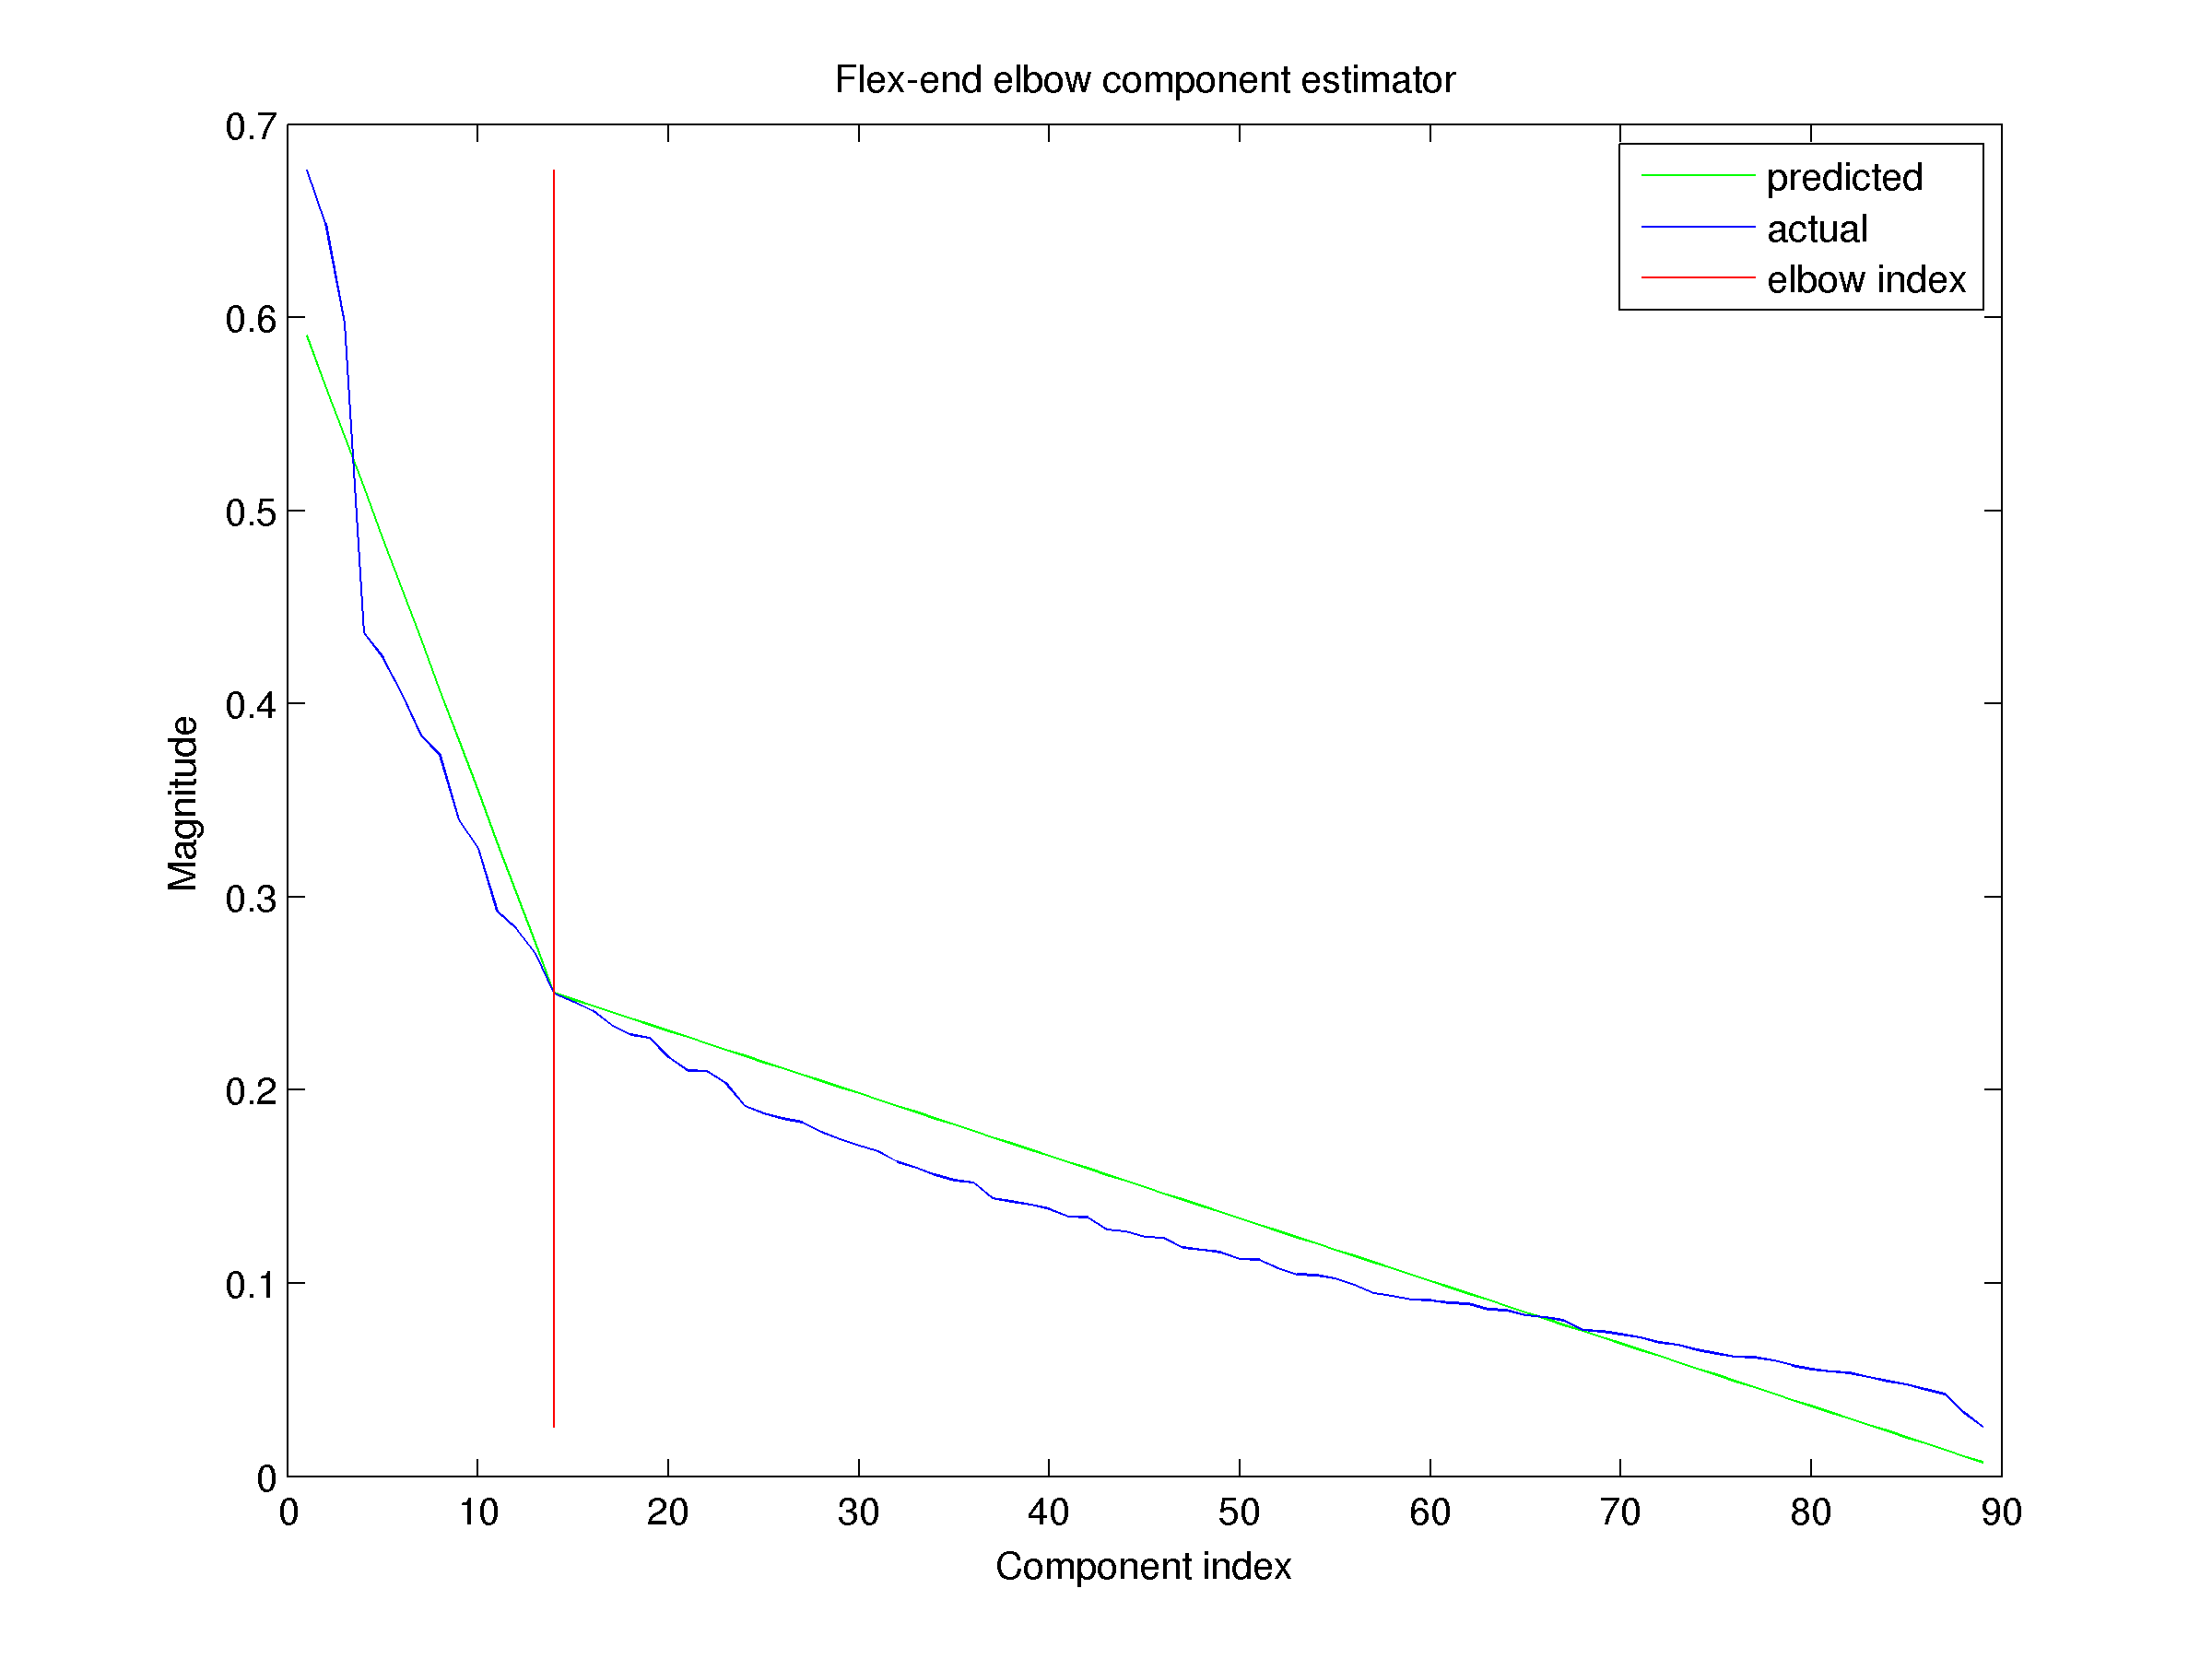
\includegraphics[width=0.9\linewidth]{100words-adj-800dim-lowercase_wmt_model-original-flex_end_elbow}
    \caption{Eigenvalues for each principal component of the 90 word vectors
    produced from the 101 word list.}
    \label{fig:101wordsunnormalizedpcaeigenvalues}
\end{figure}

\todo{switch the lambda plots in the results section to something properly labeled and scaled for easy comparison and without the elbow drawing}


Table \ref{tab:101wordsRankingsUnnormalizedPCA} gives the highest and lowest
ranking words on the first 4 principal components of the unnormalized 90 word 
vectors. A more complete list can be found in Appendix 
\ref{app:rankedwordlists:101words:unnormalized}. The eigenvalues associated 
with each component are plotted in Figure 
\ref{fig:101wordsunnormalizedpcaeigenvalues}. The eigenvalue for a component is
proportional to the fraction of variance explained by that component.


\subsection{Normalized PCA}

\begin{longtable}[!htbp]{| rllll |}
    \hline
      & \multicolumn{4}{c|}{\textbf{Component}} \\
    \textbf{Rank} & \textbf{1} & \textbf{2} & \textbf{3} & \textbf{4} \\
    \endhead
    \hline
    1 & irritable\_jj  & uncooperative\_jj  & negligent\_jj  & cold\_jj \\
    2 & uncooperative\_jj  & prompt\_jj  & uncooperative\_jj  & unreflective\_jj \\
    3 & self-pitying\_jj  & negligent\_jj  & imperturbable\_jj  & neat\_jj \\
    4 & extroverted\_jj  & systematic\_jj  & selfish\_jj  & self-pitying\_jj \\
    5 & unintelligent\_jj  & distrustful\_jj  & careless\_jj  & deep\_jj \\
    6 & talkative\_jj  & inconsistent\_jj  & prompt\_jj  & warm\_jj \\
    7 & rude\_jj  & insecure\_jj  & unreflective\_jj  & shallow\_jj \\
    \hline
    84 & steady\_jj  & uncharitable\_jj  & energetic\_jj  & thorough\_jj \\
    85 & simple\_jj  & talkative\_jj  & extroverted\_jj  & cooperative\_jj \\
    86 & systematic\_jj  & extroverted\_jj  & talkative\_jj  & talkative\_jj \\
    87 & innovative\_jj  & introspective\_jj  & pleasant\_jj  & kind\_jj \\
    88 & efficient\_jj  & energetic\_jj  & kind\_jj  & negligent\_jj \\
    89 & prompt\_jj  & considerate\_jj  & warm\_jj  & uncooperative\_jj \\
    90 & thorough\_jj  & imperturbable\_jj  & considerate\_jj  & considerate\_jj \\
    \hline
    \caption{\todo{need to caption the table for 100words-adj-800dim-lowercase\_wmt\_model-zscore\_transformed-summary\_table.tex} } \\
\end{longtable}


\begin{figure}[!htbp]
    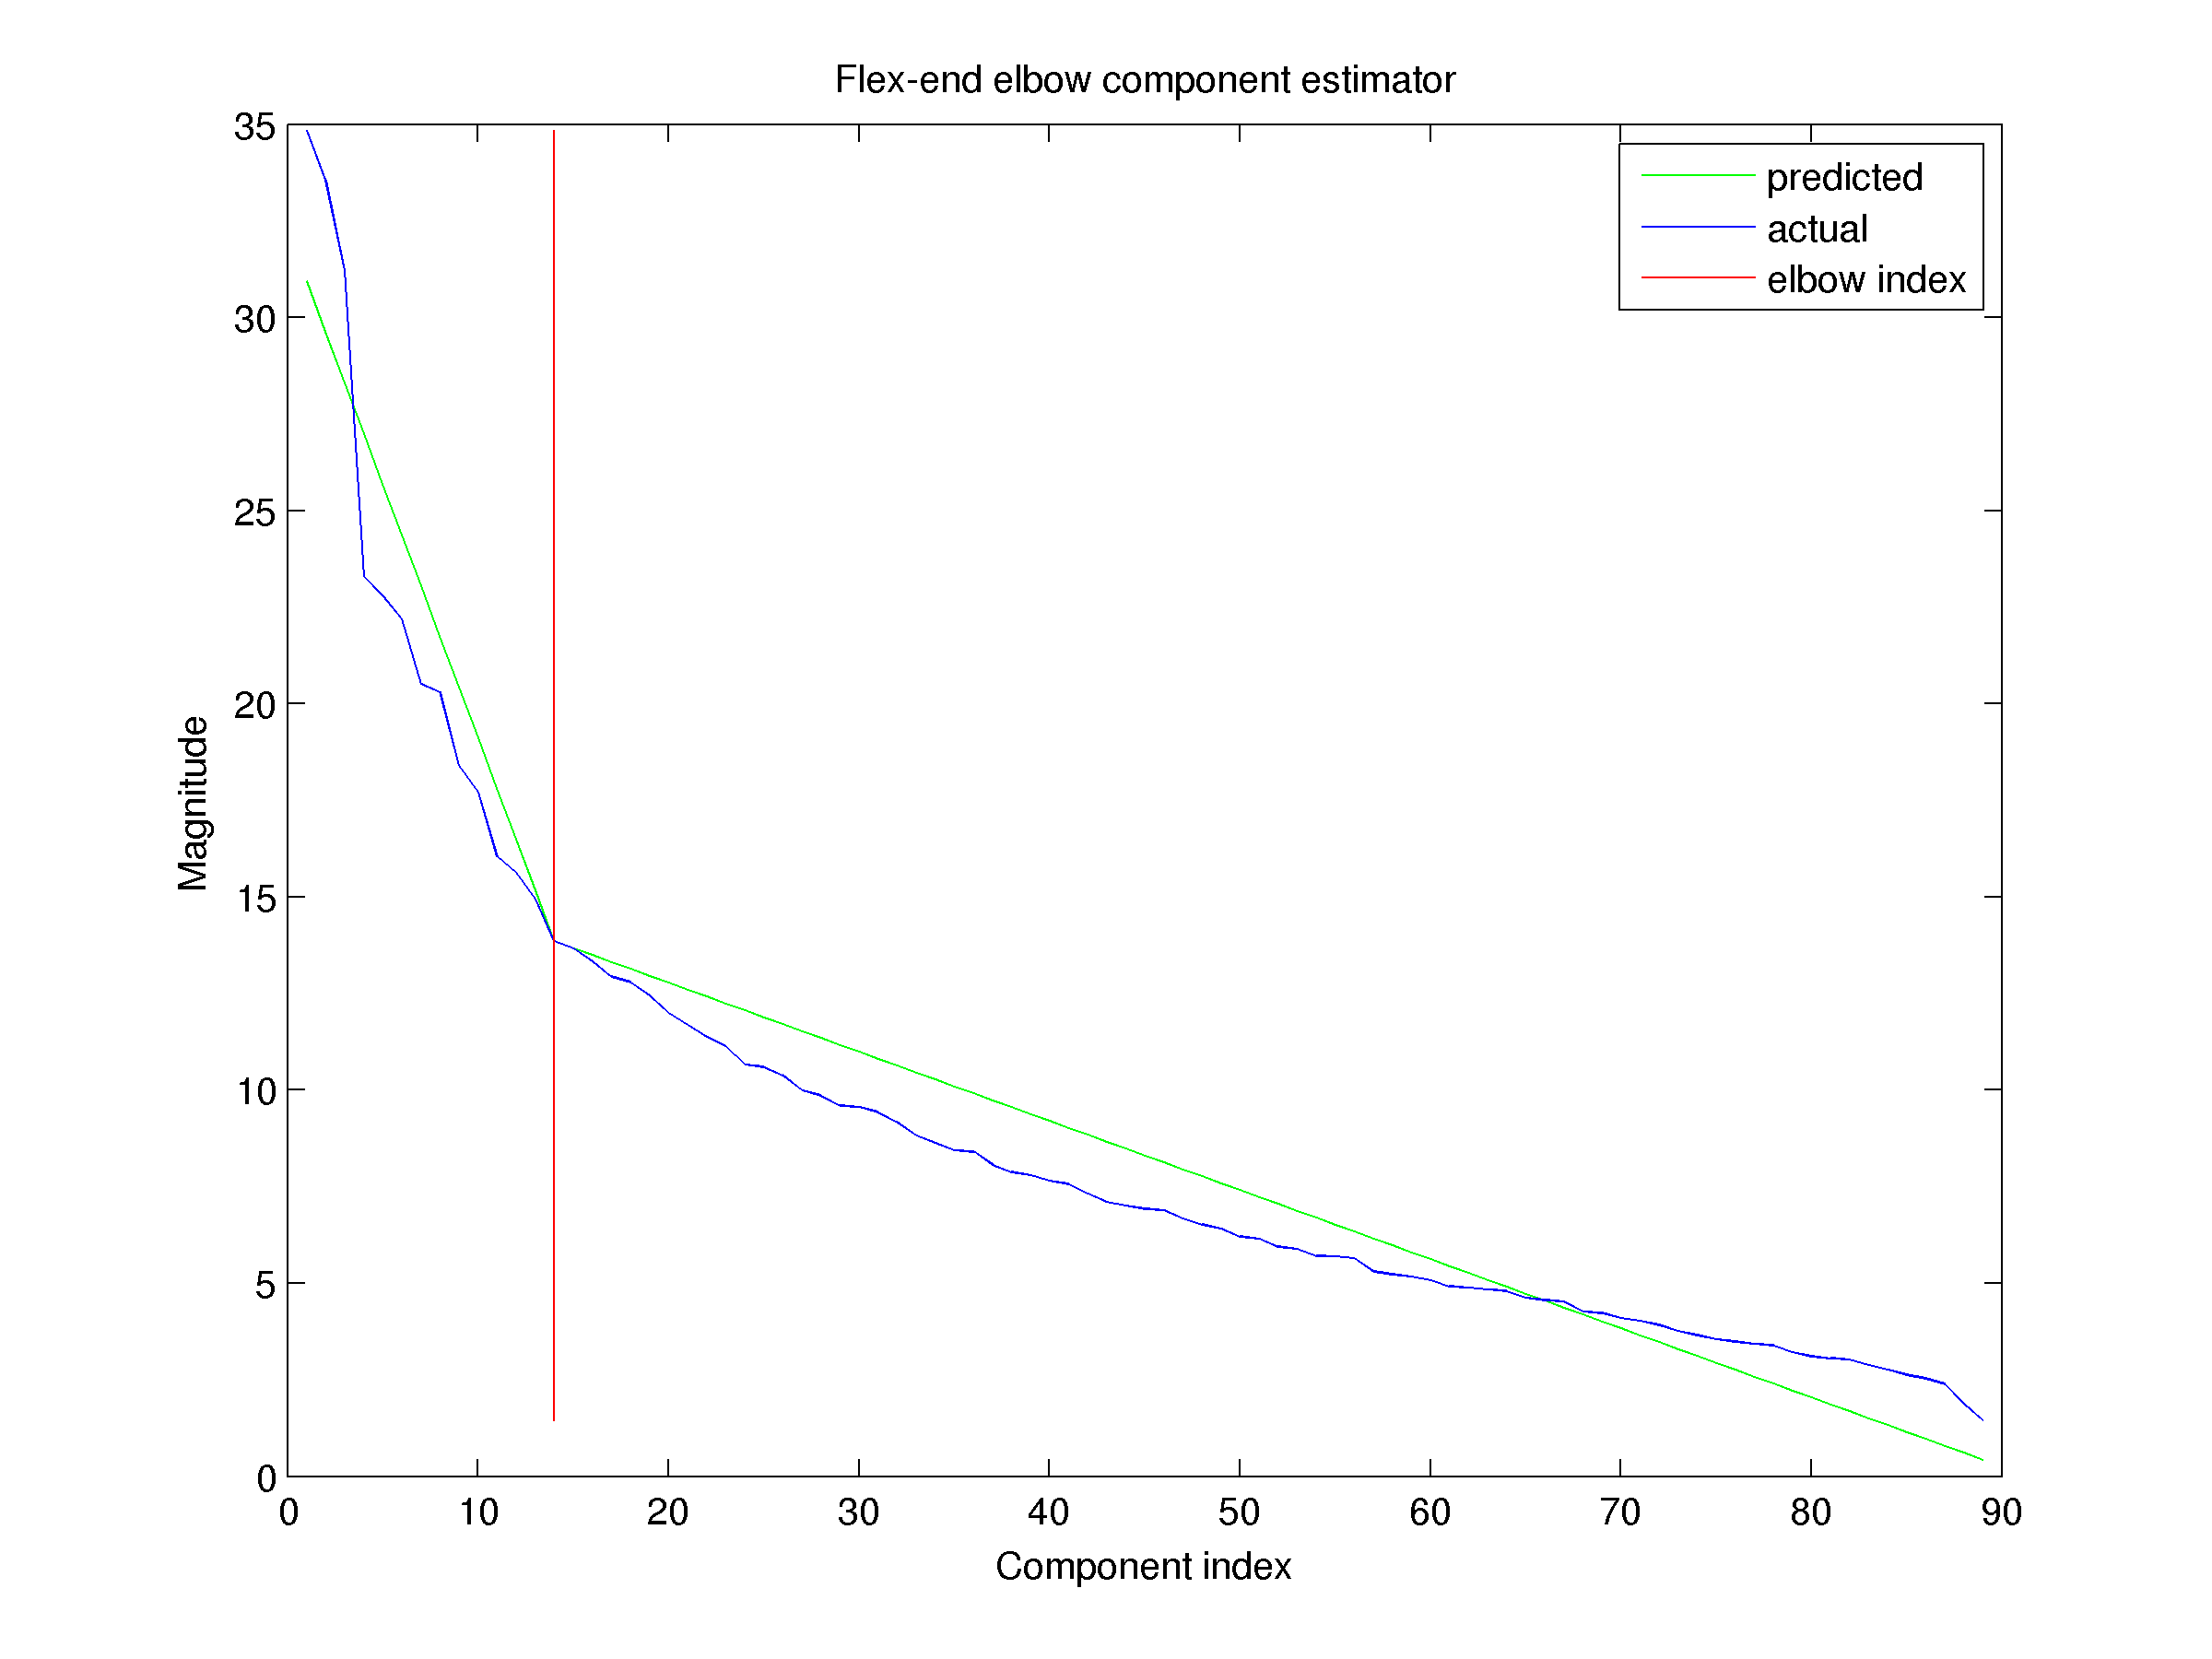
\includegraphics[width=0.9\linewidth]{100words-adj-800dim-lowercase_wmt_model-zscore_transformed-flex_end_elbow}
    \caption{Eigenvalues for each principal component of the 90 word vectors
    produced from the 101 word list after transforming to z-scores.}
    \label{fig:101wordsnormalizedpcaeigenvalues}
\end{figure}

Table \ref{tab:101wordsRankingsNormalizedPCA} gives the highest and lowest
ranking words on the first 4 principal components of the normalized 90 word 
vectors. A more complete list can be found in Appendix 
\ref{app:rankedwordlists:101words:normalized}. The eigenvalues associated 
with each component are plotted in Figure 
\ref{fig:101wordsnormalizedpcaeigenvalues}. The eigenvalue for a component is
proportional to the fraction of variance explained by that component.


\subsection{MDS}


\begin{table}[!htbp]
    \begin{tabular}{| rllll | }
        \hline
         & \multicolumn{4}{c|}{\textbf{Component}} \\
        \textbf{Rank} & \textbf{1} & \textbf{2} & \textbf{3} & \textbf{4} \\
        \hline
        1 & envious & energetic & imaginative & active \\
        2 & jealous & considerate & artistic & cooperative \\
        3 & self-pitying & introspective  & innovative & efficient \\
        4 & unkind & pleasant & unreflective & sympathetic \\
        5 & bashful & creative & unadventurous & assertive \\
        6 & fretful & imaginative & unimaginative & unsympathetic \\
        7 & uncharitable & extroverted & creative & distrustful \\
        \hline
        84 & systematic & uncooperative & careful & bright \\
        85 & thorough & inefficient & quiet & steady \\
        86 & efficient & systematic & warm & shallow \\
        87 & complex & sloppy & cold & warm \\
        88 & simple & inconsistent & fearful & neat \\
        89 & practical & unsystematic & anxious & deep \\
        90 & innovative & negligent & nervous & cold \\
        \hline
    \end{tabular}
    \caption{The highest and lowest ranking words on the first 4 components 
    derived from performing MDS on the 90 word vectors.}
    \label{tab:101wordsRankingsMDS}
\end{table}

\begin{figure}[!htbp]
    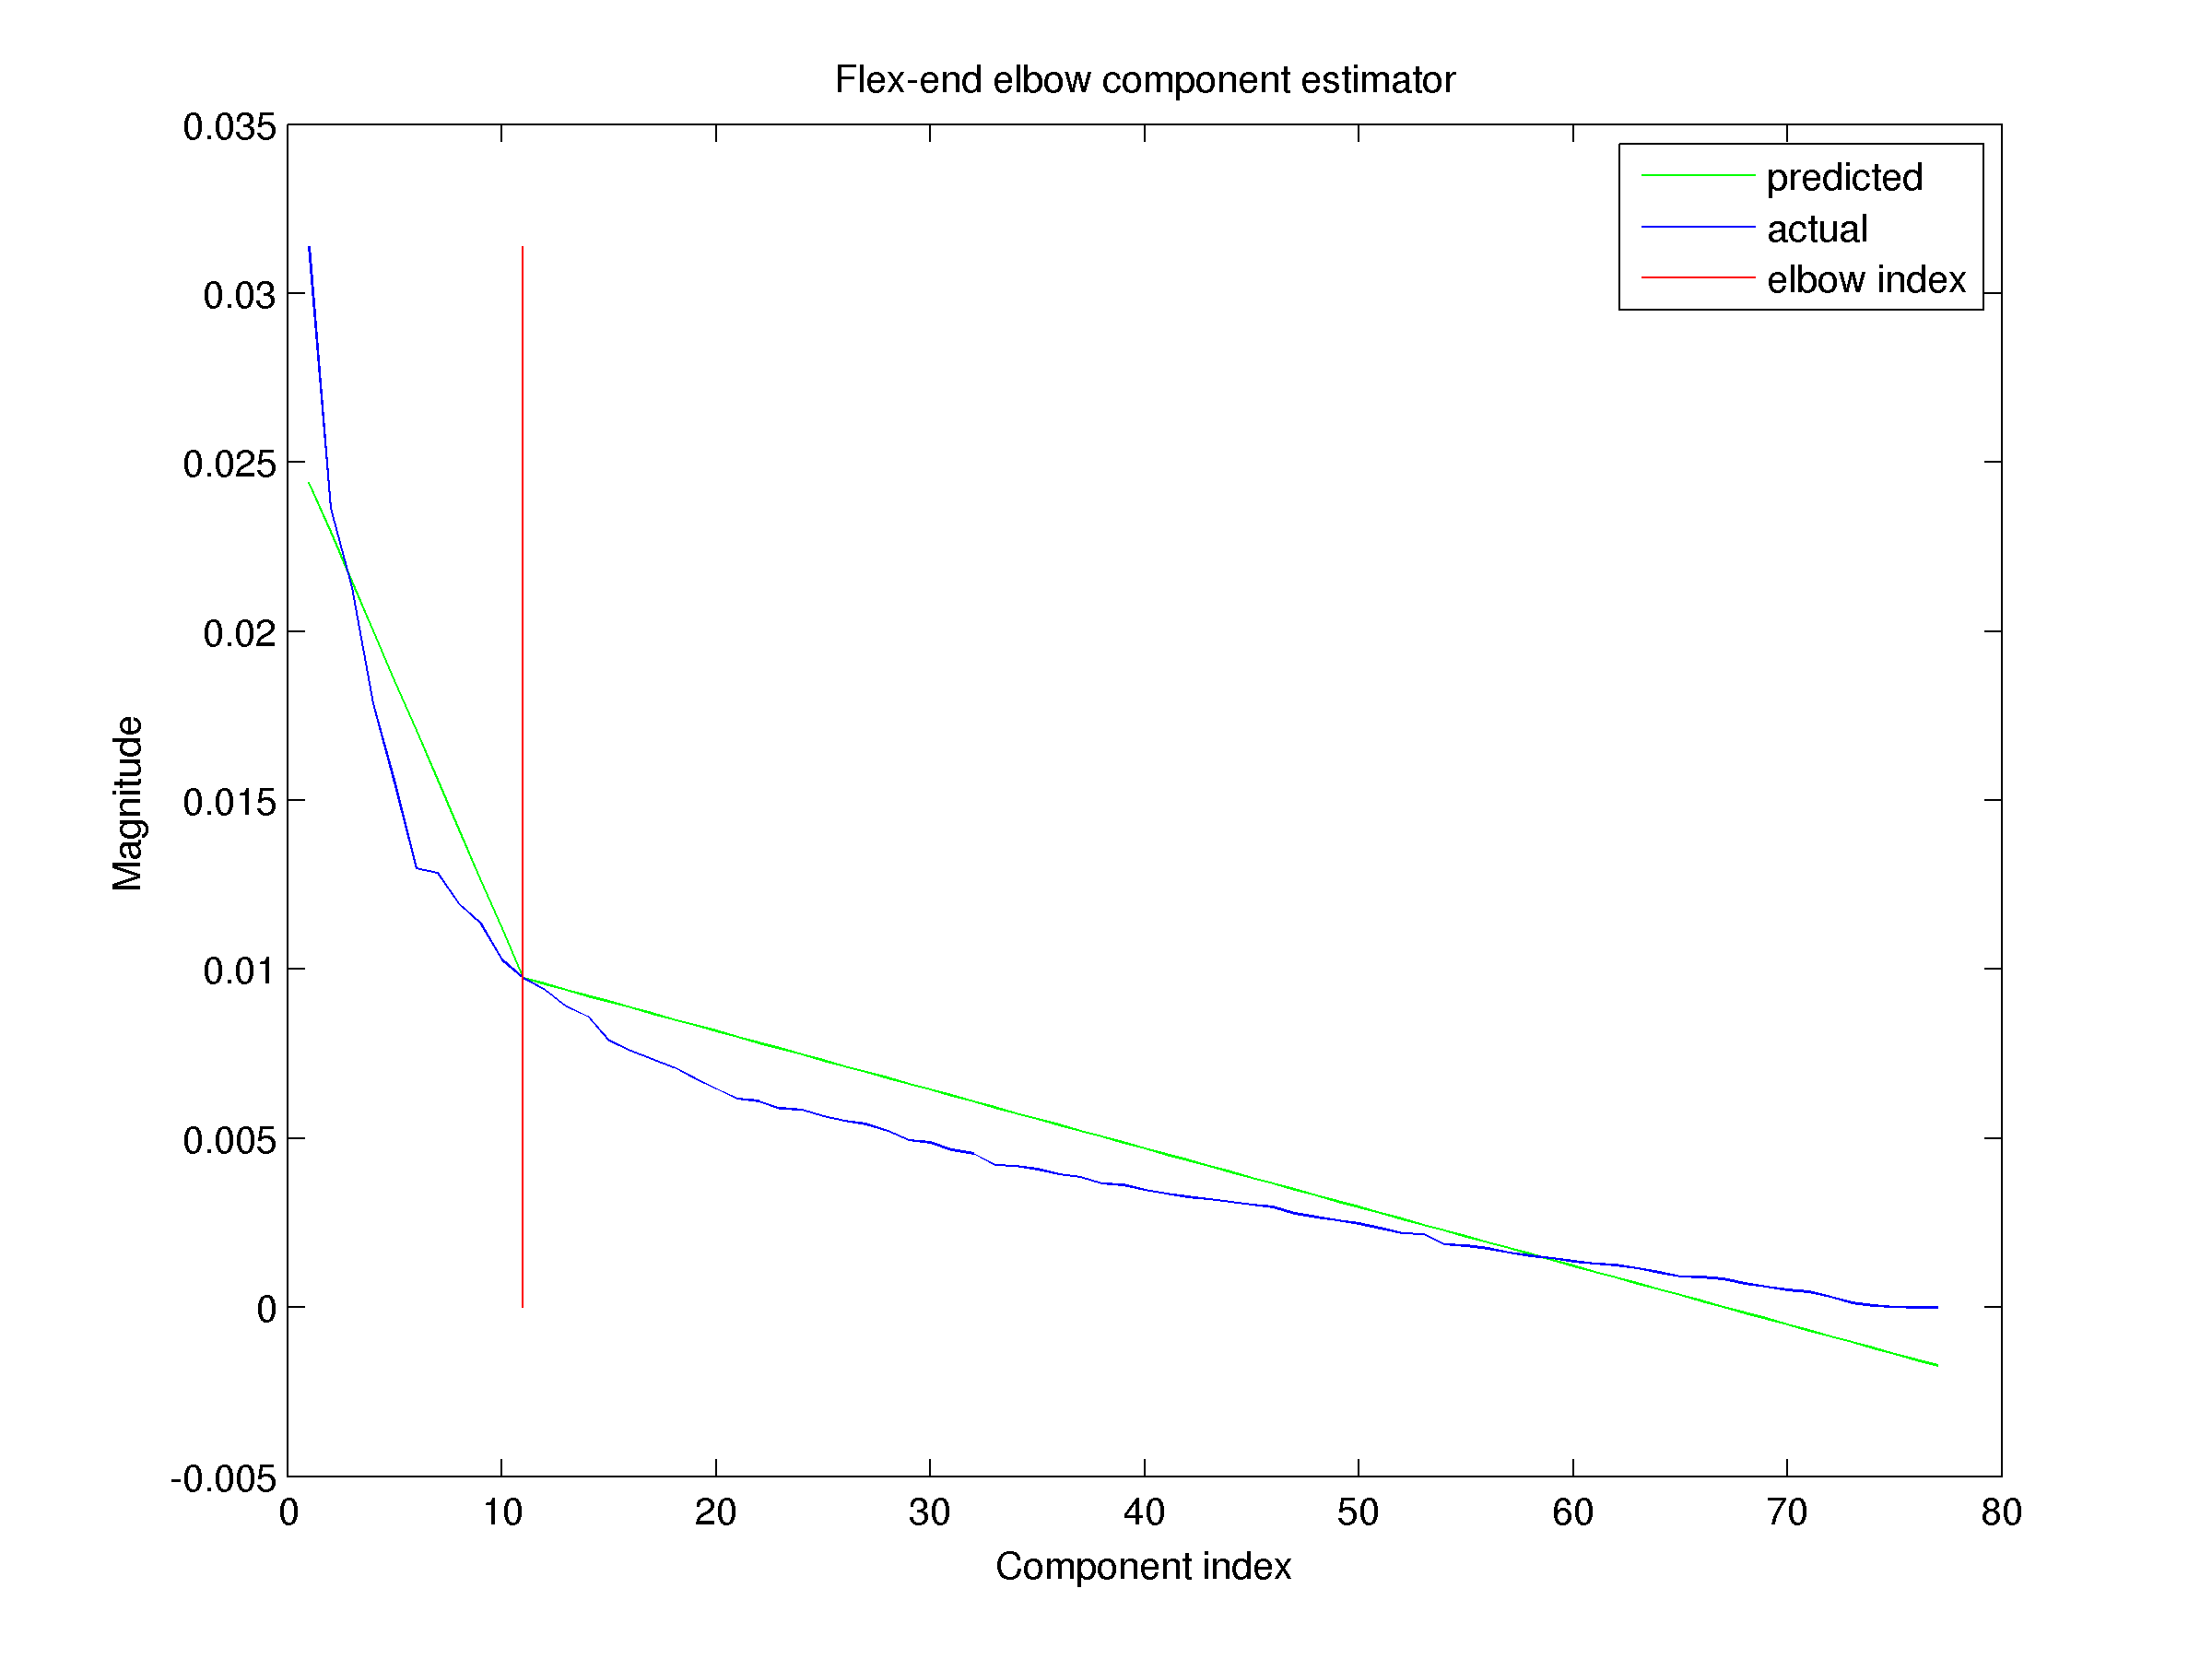
\includegraphics[width=0.9\linewidth]{100words-adj-800dim-lowercase_wmt_model-mds_transformed-flex_end_elbow}
    \caption{Eigenvalues for each principal component of the 90 word vectors
    produced from the 101 word list after multidimensional scaling.}
    \label{fig:101wordsmdseigenvalues}
\end{figure}

Table \ref{tab:101wordsRankingsMDS} gives the highest and lowest
ranking words on the first 4 principal components of the 90 word 
vectors after MDS. A more complete list can be found in Appendix 
\ref{app:rankedwordlists:101words:mds}. The eigenvalues associated 
with each component are plotted in Figure 
\ref{fig:101wordsmdseigenvalues}. The eigenvalue for a component is
proportional to the fraction of variance explained by that component.


\section{438 word set}

\todo{remember to mention how many and which words of the hundred actually appeared in the corpus - and thus had a vector representation}

\subsection{Unnormalized PCA}

\begin{table}[!htbp]
    \begin{tabular}{| rllll | }
        \hline
         & \multicolumn{4}{c|}{\textbf{Component}} \\
        \textbf{Rank} & \textbf{1} & \textbf{2} & \textbf{3} & \textbf{4} \\
        \hline
        1 &  &  &  &  \\
        2 &  &  &  &  \\
        3 &  &  &  &  \\
        4 &  &  &  &  \\
        5 &  &  &  &  \\
        6 &  &  &  &  \\
        7 &  &  &  &  \\
        \hline
        84 &  &  &  &  \\
        85 &  &  &  &  \\
        86 &  &  &  &  \\
        87 &  &  &  &  \\
        88 &  &  &  &  \\
        89 &  &  &  &  \\
        90 &  &  &  &  \\
        \hline
    \end{tabular}
    \caption{The highest and lowest ranking words on the first 4 components 
    derived from unnormalized PCA of the 90 word vectors.}
    \label{tab:438wordsRankingsUnnormalizedPCA}
\end{table}

Table \ref{tab:438wordsRankingsUnnormalizedPCA} gives the highest and lowest
ranking words on the first 4 principal components of the unnormalized 90 word 
vectors. A more complete list can be found in Appendix 
\ref{app:rankedwordlists:438words:unnormalized}.


\subsection{Normalized PCA}

\begin{table}[!htbp]
    \begin{tabular}{| rllll | }
        \hline
         & \multicolumn{4}{c|}{\textbf{Component}} \\
        \textbf{Rank} & \textbf{1} & \textbf{2} & \textbf{3} & \textbf{4} \\
        \hline
        1 &  &  &  &  \\
        2 &  &  &  &  \\
        3 &  &  &  &  \\
        4 &  &  &  &  \\
        5 &  &  &  &  \\
        6 &  &  &  &  \\
        7 &  &  &  &  \\
        \hline
        84 &  &  &  &  \\
        85 &  &  &  &  \\
        86 &  &  &  &  \\
        87 &  &  &  &  \\
        88 &  &  &  &  \\
        89 &  &  &  &  \\
        90 &  &  &  &  \\
        \hline
    \end{tabular}
    \caption{The highest and lowest ranking words on the first 4 components 
    derived from normalized PCA of the 90 word vectors.}
    \label{tab:438wordsRankingsNormalizedPCA}
\end{table}

Table \ref{tab:438wordsRankingsNormalizedPCA} gives the highest and lowest
ranking words on the first 4 principal components of the normalized 90 word 
vectors. A more complete list can be found in Appendix 
\ref{app:rankedwordlists:438words:normalized}.


\subsection{MDS}


\begin{table}[!htbp]
    \begin{tabular}{| rllll | }
        \hline
         & \multicolumn{4}{c|}{\textbf{Component}} \\
        \textbf{Rank} & \textbf{1} & \textbf{2} & \textbf{3} & \textbf{4} \\
        \hline
        1 &  &  &  &  \\
        2 &  &  &  &  \\
        3 &  &  &  &  \\
        4 &  &  &  &  \\
        5 &  &  &  &  \\
        6 &  &  &  &  \\
        7 &  &  &  &  \\
        \hline
        84 &  &  &  &  \\
        85 &  &  &  &  \\
        86 &  &  &  &  \\
        87 &  &  &  &  \\
        88 &  &  &  &  \\
        89 &  &  &  &  \\
        90 &  &  &  &  \\
        \hline
    \end{tabular}
    \caption{The highest and lowest ranking words on the first 4 components 
    derived from performaing MDS on the 90 word vectors.}
    \label{tab:438wordsRankingsMDS}
\end{table}

Table \ref{tab:438wordsRankingsMDS} gives the highest and lowest
ranking words on the first 4 principal components of the 90 word 
vectors after MDS. A more complete list can be found in Appendix 
\ref{app:rankedwordlists:438words:mds}.

\section{101 and 438 word sets combined}

\todo{remember to mention how many and which words actually appeared in the corpus - and thus had a vector representation}
\todo{check for copy-paste errors on the tables, their captions, and the references}

\subsection{Unnormalized PCA}

\begin{table}[!htbp]
    \begin{tabular}{| rllll | }
        \hline
         & \multicolumn{4}{c|}{\textbf{Component}} \\
        \textbf{Rank} & \textbf{1} & \textbf{2} & \textbf{3} & \textbf{4} \\
        \hline
        1 &  &  &  &  \\
        2 &  &  &  &  \\
        3 &  &  &  &  \\
        4 &  &  &  &  \\
        5 &  &  &  &  \\
        6 &  &  &  &  \\
        7 &  &  &  &  \\
        \hline
        84 &  &  &  &  \\
        85 &  &  &  &  \\
        86 &  &  &  &  \\
        87 &  &  &  &  \\
        88 &  &  &  &  \\
        89 &  &  &  &  \\
        90 &  &  &  &  \\
        \hline
    \end{tabular}
    \caption{The highest and lowest ranking words on the first 4 components 
    derived from unnormalized PCA of the 90 word vectors.}
    \label{tab:438and101wordsRankingsUnnormalizedPCA}
\end{table}

Table \ref{tab:438and101wordsRankingsUnnormalizedPCA} gives the highest and lowest
ranking words on the first 4 principal components of the unnormalized 90 word 
vectors. A more complete list can be found in Appendix 
\ref{app:rankedwordlists:438and101words:unnormalized}.


\subsection{Normalized PCA}

\begin{table}[!htbp]
    \begin{tabular}{| rllll | }
        \hline
         & \multicolumn{4}{c|}{\textbf{Component}} \\
        \textbf{Rank} & \textbf{1} & \textbf{2} & \textbf{3} & \textbf{4} \\
        \hline
        1 &  &  &  &  \\
        2 &  &  &  &  \\
        3 &  &  &  &  \\
        4 &  &  &  &  \\
        5 &  &  &  &  \\
        6 &  &  &  &  \\
        7 &  &  &  &  \\
        \hline
        84 &  &  &  &  \\
        85 &  &  &  &  \\
        86 &  &  &  &  \\
        87 &  &  &  &  \\
        88 &  &  &  &  \\
        89 &  &  &  &  \\
        90 &  &  &  &  \\
        \hline
    \end{tabular}
    \caption{The highest and lowest ranking words on the first 4 components 
    derived from normalized PCA of the 90 word vectors.}
    \label{tab:438and101wordsRankingsNormalizedPCA}
\end{table}

Table \ref{tab:438and101wordsRankingsNormalizedPCA} gives the highest and lowest
ranking words on the first 4 principal components of the normalized 90 word 
vectors. A more complete list can be found in Appendix 
\ref{app:rankedwordlists:438and101words:normalized}.


\subsection{MDS}


\begin{table}[!htbp]
    \begin{tabular}{| rllll | }
        \hline
         & \multicolumn{4}{c|}{\textbf{Component}} \\
        \textbf{Rank} & \textbf{1} & \textbf{2} & \textbf{3} & \textbf{4} \\
        \hline
        1 &  &  &  &  \\
        2 &  &  &  &  \\
        3 &  &  &  &  \\
        4 &  &  &  &  \\
        5 &  &  &  &  \\
        6 &  &  &  &  \\
        7 &  &  &  &  \\
        \hline
        84 &  &  &  &  \\
        85 &  &  &  &  \\
        86 &  &  &  &  \\
        87 &  &  &  &  \\
        88 &  &  &  &  \\
        89 &  &  &  &  \\
        90 &  &  &  &  \\
        \hline
    \end{tabular}
    \caption{The highest and lowest ranking words on the first 4 components 
    derived from performaing MDS on the 90 word vectors.}
    \label{tab:438and101wordsRankingsMDS}
\end{table}

Table \ref{tab:438and101wordsRankingsMDS} gives the highest and lowest
ranking words on the first 4 principal components of the 90 word 
vectors after MDS. A more complete list can be found in Appendix 
\ref{app:rankedwordlists:438and101words:mds}.


\chapter{Discussion}

\section{Not what we expected}

\section{Could it be the corpus?}

WMT11 is a news corpus. Possibly its topic matter does not focus on people enough for those word senses to be properly represented. There are other, smaller, corpora with much broader language representation - for example, the brown corpus is a well known and freely available million word corpus. The British National Corpus is in the hundreds of millions of words and was created to be very broad-based. Additionally, there are spoken-language corpora like MICASE (Michigan Corpus of Academic Spoken English) and CPSA (Corpus of Spoken Professional American-English). These corpora could be used by themselves or potentially improved by using a model derived from a large news corpus like WMT11 or Gigaword as a starting point and then training on the smaller corpus.

\section{Could it be polysemy?}

\section{Could the dimensions be non-personality attributes?}
\section{Could the dimensions not be scaled on personality-ness?}

\todo{What I mean here is that the dimensions could be things like ``suitability to describe warmth'' both cold and warm would score highly but organized would score low.}

\section{Could the number of dimensions in the lexical model be affecting things?}

\section{Could the personality meanings not be being captured?}

\todo{This may be part of the previous - too few or too many dimensions might elide the personality dimensions}

\section{Could the problem be an underlying nonlinear structure?}

\section{Could the problem be the nonlinear transformation from cosine to Euclidean topology?}

\chapter{Future Work}

\section{Rerun on other corpora}

\subsection{Gigaword}
\subsection{Smaller corpora}
\subsection{Small corpus from large starting point}

\section{Examine technique for detecting word usage shift between corpora}

\todo{Turn text summary of method below into more final version for future work}
Train model 1 on corpus 1. Save model 1. Train model 2 on corpus 2 using model 1 as a starting point. Align the two models (using words common to the two corpora and a loss function that depends on how many different words you expect (for example, if you will use $L^p$ norms\footnote{An $L^p$ norm calculates the length of an n-dimensional vector $x$ as $\|x\|_p=\left(|x_1|^p+|x_2|^p+\dotsb+|x_n|^p\right)^{\frac{1}{p}}$} and subtraction to calculate distance, you can use a lower $p$ exponent for a lower proportion of expected differences).

\section{Perform modeling in Euclidean topology}

\todo{Turn summary into final form}
Because the vectors must be converted to use Euclidean distances before PCA will work correctly, the principal components are not components of the vectors in cosine distance space. Thus, we can only rank the personality words and it is impossible to look for dimensions whose meaning will not be obvious based on ranking the personality words.

One approach would be to transform all the words. However the distance matrix alone would be enormous (5 hundred thousand words would require 250 billion distances). Since most modern MDS implementations use some form of gradient descent under the hood, I considered using stochastic gradient descent with the distance matrix being implicit in the original point values. The initial point for the descent could be the original point values since Euclidean and cosine distances are similar. However, that is a very special-purpose application of MDS. Since it could be hard to code due to the sizes of the data involved, and would only give an approximation of the best point locations, I don't think it is worth the effort at this time.

I think it is better to rewrite the training section of the skip-gram to use Euclidean rather than cosine distance. This modification will increase training time by a constant factor, but I would hope that factor is small.

\section{Do the big-5 etc. personality dimensions come out of a pseudo-personality test?}
\todo{Turn summary into final form}
What I mean is if you count the frequency for which different personality adjectives are used to describe different named person-entities in the corpus, do you get the same descriptive dimensions as you do for when you ask people to rate others on n dimensions.

\section{What happens if you tag personality words when they are referring to a specific person?}

\section{Use perplexity to calculate the number of personality dimensions}

\appendix
\chapter{Scripts used in preprocessing}
\section{Text of filter\_angle\_tags.pl}
\label{app:filterangletags}
\lstset{language=Perl}
\begin{lstlisting}
#!/usr/bin/perl
use strict;
use warnings;

#######################
# Usage: filter_angle_tags.pl < source > dest
# or:    filter_angle_tags.pl source1 source2 > filtered
#
# Remove stray html, urls and stock symbols to prepare
# for tagging

my $has_bracket_pair = qr!<[A-z/][^<>]*>!;
my $bracket_pair_split = qr!($has_bracket_pair)!;
my $html_string = q(<span |<strong>|</strong>|).
    q(<em>|</em>|<[bauipq]>|</[pqbaui]>|<\s*br\s*/?>|).
    q(<\s*/br\s*>|<p\s*/?>|</?h.>|</?blockquote|).
    q(</?code>|<font[ >]|</font|</?acronym|</?strike|).
    q(</?cite|</?q |</>|</?abbr |</?del |<javascript|).
    q(</?itals>|</?script|</?center>|<SPEAKER );
my $html_regex = qr(${html_string});

sub keep_segment{
    my ($seg) = @_;
    return !($seg =~ m!$has_bracket_pair!) or !(
        $seg =~ m(http://) or
        $seg =~ m(href) or
        $seg =~ m(\.com\W|\.gov\W) or
        $seg =~ m(${html_regex}) or
        $seg =~ m(<[A-z0-9]{0,9}[.=/][A-Z0-9]{0,6}>) or
        $seg =~ m(<CF7[01]>) or
        $seg =~ m(<ID:[A-z0-9]+>)
        );
}

while(<>){
    chomp;
    if (m/$has_bracket_pair/) {
        my @segments = split($bracket_pair_split, $_);
        @segments = grep( &keep_segment($_), 
                          @segments);
        print join(" ", @segments),"\n" 
            if (@segments);
    }else{
        print "$_\n";
    }

}
\end{lstlisting}

\section{Text of tag\_corpus.sh}
\label{app:tagcorpus}
\lstset{language=sh}
\begin{lstlisting}
#!/bin/bash

############
# Script I used to tag the WMT11 corpus - it needed to
# be split because the TreeTagger tokenizer reads
# everything into memory.

# The data file for the cleaned data
WMT11=/mnt/linux_data/wmt11_no_angle_tags.txt

# The prefix used for split files
SPLIT_FILENAME=/mnt/linux_data/wmt11_no_angle_split

# Data file for the tagged data
TAGGED_WMT11=/mnt/linux_data/wmt11_tagged.txt

# Put treetagger on path
PATH="$PATH:/home/eric/SW/TreeTagger/cmd:"\
"/home/eric/SW/TreeTagger/bin:."

# Split into 10,000,000 lines per file (about 1.5GiB
# per)
if [ -f ${SPLIT_FILENAME}aa ]; then 
    echo "Not splitting again. Split already exists"
else
    split -l10000000 "$WMT11" "$SPLIT_FILENAME"
fi

# Tag the split files
if [ -f "$TAGGED_WMT11" ]; then 
    echo "Not tagging again. Tagged file "\
         "already exists"
else
    for i in ${SPLIT_FILENAME}*; do
        echo "Tagging $i"
        tree-tagger-english-utf8 $i | \
            reassemble_tags.pl >> "$TAGGED_WMT11"
    done
fi
\end{lstlisting}

\section{Text of reassemble\_tags.pl}
\label{app:reassembletags}
\lstset{language=Perl}
\begin{lstlisting}
#!/usr/bin/perl
use strict;
use warnings;

################
# Usage: reassemble_tags.pl < tagged.txt
#
# Takes tagged text from treetagger and reassembles it
# into 1 sentence per line (multiple sentence ending
# tags are kept on the same line)

# Tracks whether the previous tag was a sentence-ender
# in order to tell where to end the lines.
my $last_tag_was_sentence=(1==0);

# Combine words and sentences
while(<>){
    my ($word, $tag) = split('\t');
    if(defined($tag)){
        # End the line if transitioning from "SENT" to
        # another tag
        my $tag_is_sentence = $tag eq "SENT";
        if ($last_tag_was_sentence && !$tag_is_sentence){
            print "\n";
        }

        # Output the word with its tag
        if(defined($word)){
            print "${word}_${tag} ";
        }else{
            print "${word}_unknown_tag ";
        }

        # Update last tag state variable
        $last_tag_was_sentence = $tag_is_sentence;
    }
}

# If the last tag in the file was a sentence tag,
# output a newline
if ($last_tag_was_sentence){
    print "\n";
}
\end{lstlisting}

\chapter{Scripts used in analysis}

\section{extract\_vectors.py}
\label{app:extractvectors}
\lstset{language=Python}
\begin{lstlisting}
#!/usr/bin/python
from gensim.models import word2vec
import logging
import os
import csv
import sys


# Check command line arguments and print usage if
# wrong number of arguments
if len(sys.argv) != 3:
    import textwrap
    sys.stderr.write(
        "Usage: %s list_of_terms.txt "+
        "model_file.model\n" % sys.argv[0])
    sys.stderr.write("\n")
    sys.stderr.write(
        textwrap.fill(
            "Each line in list_of_terms.txt is "+
            "treated as a term. For each term, if a "+
            "corresponding term exists in the "+
            "word2vec model (generated by "+
            "word2vec.save) then that term and the "+
            "corresponding vector are printed to "+
            "stdout as a csv file"))
    sys.exit(-1)

# Command line arguments
term_list_filename = sys.argv[1]
input_model_filename = sys.argv[2]

# Set up logging
logging.basicConfig(
    format='%(asctime)s : %(levelname)s : %(message)s', 
    level=logging.INFO)

# Load the model
model = word2vec.Word2Vec.load(input_model_filename)
logging.info("Done loading input model")

# Loop through the terms, outputting appropriate
# vectors
out = csv.writer(sys.stdout)
with open(term_list_filename) as terms:
    for term in terms:
        try:
            term = term.rstrip() # Remove line-ending
            v = model.vocab[term]
            vector = model.syn0[v.index]
            vector_str = ["%.19g" % n for n in vector]
            out.writerow([term] + vector_str)
        except KeyError:
            logging.info('Skipped missing term "%s"' % 
                         term)
\end{lstlisting}


\section{Elbow point algorithms}
\label{app:elbow_point_algorithms}
\lstset{language=Matlab}

\subsection{elbow\_point.m}

\begin{lstlisting}
 function [elbow_index,best_estimate] = ...
      elbow_point(lambdas)
% Returns the index at which the slope of the lambdas
% changes
%
% In using a scree plot to discover the number of 
% principal components, a frequent method is to choose
% the "elbow", the inflection point of the curve. One
% way of formalizing this is approximating the scree 
% plot with two lines. One goes from the  beginning to
% the elbow point and the other to the end. Whichever
% is closest is the best elbow point 
%
% Exhaustive search for the best approximation of
% the function composed of the ordered pairs
% i,lambdas(i) composed of the lines
% (1,lambdas(1))...(i,lambdas(i)) and
% ((i,lambdas(i)...(end, lambdas(end))
%
% Mean absolute value of the difference is used as
% the measure of goodness of fit
%
% best_estimate - the linear fit to the lambdas
% implied by elbow_index

if size(lambdas,1) > 1
    lambdas = lambdas';
end
best = 1;
best_error = inf;
best_estimate = [];
for cur=1:length(lambdas)
    cur_estimate_a = linspace(lambdas(1), ...
         lambdas(cur), cur);
    cur_estimate_b = linspace(lambdas(cur), ...
         lambdas(end), length(lambdas)-cur+1);
    cur_estimate = [cur_estimate_a(1:end-1), ...
         cur_estimate_b];
    cur_error=mean(abs(cur_estimate - lambdas));
    if cur_error < best_error
        best_error = cur_error;
        best = cur;
        best_estimate = cur_estimate;
    end
end

elbow_index = best;

end
\end{lstlisting}

\subsection{flex\_end\_elbow\_point.m}
\begin{lstlisting}
 function [elbow_index,best_estimate] = ...
      flex_end_elbow_point(lambdas)
% Returns the index at which the slope of the lambdas
% changes
%
% In using a scree plot to discover the number of
% principal components, a frequent method is to
% choose the "elbow", the inflection point of the
% curve. One way of formalizing this is approximating
% the scree plot with two lines. One goes from the
% beginning to the elbow point and the other to the
% end. Whichever is closest is the best elbow point.
%
% This code is similar to elbow_point except that the
% height at the ends is adjustable. This frequently
% leads to a more conservative estimate of when the
% slope changes and a closer approximation of the
% lambdas. I think it is more like what humans do than
% offset_elbow_point.
%
% Exhaustive search for the best approximation of the
% function composed of the ordered pairs i,lambdas(i)
% composed of the lines (1,height_1)...(i,lambdas(i))
% and ((i,lambdas(i)...(end, height_end)
%
% Mean squared difference is used as the measure of
% goodness of fit. (It looks more like what a human
% would do than the mean abs used in other
% elbow_point versions.)
%
% best_estimate - the linear fit to the lambdas
% implied by elbow_index

if size(lambdas,1) > 1
    lambdas = lambdas';
end
best = 1;
best_error = inf;
best_estimate = [];
for cur=1:length(lambdas)
    % Since the two lines are independent, we can
    % minimize them in sequence. I minimize the error
    % on the first line, holding the second constant
    % then minimize the second line holding the first
    % at the optimum found in the first pass
    [h1, ~]=fminbnd(@(h) linpredict([h,lambdas(end)]),...
         lambdas(cur), max(lambdas));
    [~, cur_error]=fminbnd(@(h) linpredict([h1,h]),...
         -max(lambdas), lambdas(cur));
    if cur_error < best_error
        best_error = cur_error;
        best = cur;
        best_estimate = cur_estimate;
    end
end

elbow_index = best;

    % Calculate the two-line fit with the elbow_index
    % at cur and the heights at the beginning and end
    % set to heights(1) and heights(2) Also sets
    % cur_estimate and uses lambdas
    function err=linpredict(heights)
        cur_estimate_a = linspace(heights(1),...
             lambdas(cur), cur);
        cur_estimate_b = linspace(lambdas(cur), ...
             heights(2), length(lambdas)-cur+1);
        cur_estimate = [cur_estimate_a(1:end-1),...
             cur_estimate_b];
        err=mean(abs(cur_estimate - lambdas).^2);
    end

end
\end{lstlisting}

\subsection{log\_scree\_elbow.m}
\begin{lstlisting}
function [elbow_index,best_x1, best_x2, predicted] = ...
     log_scree_elbow( lambdas, min_dist )
% Looks for the line in the log(lambdas) that has the
% most inliers, then counts the first outlier as the
% elbow
%
% Scree plots of random stuff look like exponential
% curves. Thus, they are flat on a log scale. The
% dimensions carrying information either have a
% different slope or aren't exponential at all. Thus,
% they will be outliers. On a log plot, the random
% stuff looks like a straight line. (However, if
% the system is rank deficient, the last few principal
% components will sharply trail off and not look like
% a straight line.)
% 
% Let lambdas be the 'latent' return from princomp.
% 
% I fit an exponential to the end-points of all
% sufficiently large sub-intervals of the lambda
% values. I choose the interval whose error looks the
% most like Gaussian noise (that is, has the lowest
% test statistic for a Jarque-Bera). Then I fit an
% exponential to all those points and calculate the
% standard deviation of the errors. Finally, the
% first point with an error less than 3 standard
% deviations, I count as the first random point. All
% points before that are outliers and I count the
% last of the outlier points as my elbow index.
%
% lambdas - a vector of strictly postitive scalars
%     sorted in decreasing order. The 'latent'
%     return from princomp
%
% min_dist - the minimum length interval to be
%     considered as a potential "all-random" interval.
%     The smaller this is, the less power the
%     normality test has. However, it cannot be larger
%     than the number of random values that are
%     decreasing exponentially. The default is
%     length(lambdas)/4

if any(lambdas <= 0)
    error('log_scree_elbow:pos_lambda',...
        ['All lambda values must be strictly '...
        'positive in log_scree_elbow']);
end

if ~exist('min_dist','var')
    min_dist = ceil(length(lambdas)/4);
end

if min_dist < 2
    error('log_scree_elbow:min_dist_too_small',...
        ['min_dist parameter to log_scree_elbow '...
        'must be at least 2.']);
end
        

if length(lambdas)-min_dist < 20 % This is a fudge
                  % factor, but if it is less than 
                  % 20, there are way too few points
    error('log_scree_elbow:not_enough_points',...
        ['There must be at least 20 more lambda '...
        'values than min distance']);
end

if size(lambdas, 1) > 1
    lambdas = lambdas';
end

% Loop two indices x1 and x2 through the lambdas,
% fitting an exponential and finding outliers
n=length(lambdas);
best_x1 = 1;
best_x2 = 1+min_dist;
best_normality_test_stat = inf;
warning('off','stats:jbtest:PTooBig');
warning('off','stats:jbtest:PTooSmall');
for x1=1:n
    y1=lambdas(x1);
    for x2=(x1+min_dist+1):n
        % Fit an exponential to these two points
        y2=lambdas(x2);
        b=(-log(y1)+log(y2))/(-x1+x2);
        a=y1/exp(b*x1);

        % Calculate the errors for that exponential
        predicted=a.*exp(b.*(1:n));
        errors = lambdas-predicted;

        % Calculate the degree to which the errors in
        % that interval match the normal distribution.
        % Ideally, I'd use the Anderson-Darling test
        % statistic because I am particularly
        % interested in excluding outliers from the
        % interval and it is more sensitive to them.
        % However, it is not available in R2012, so
        % I will use the Jauques-Berra test
        is_inlier = (1:n > x1) & (1:n < x2);
        [~,~,jbtest_stat]=jbtest(errors(is_inlier));
        inlier_std = std(errors(is_inlier));
        if isnan(inlier_std)
            fprintf('Nan');
        end
        % If this section looks more normal than any
        % others, call it the best
        if jbtest_stat < best_normality_test_stat
            best_normality_test_stat = jbtest_stat;
            best_x1 = x1;
            best_x2 = x2;
        end
    end
end
warning('on','stats:jbtest:PTooSmall');
warning('on','stats:jbtest:PTooBig');


% Do a least-squares fit on all the inliers
x1 = best_x1;
x2 = best_x2;
y1=lambdas(x1);
y2=lambdas(x2);
b=(-log(y1)+log(y2))/(-x1+x2);
a=y1/exp(b*x1);
is_inlier = (1:n > x1) & (1:n < x2);

xdata = find(is_inlier);
ydata = lambdas(is_inlier);
inlier_params = nlinfit(xdata, ydata, @expfun, [a,b]);

% Calculate the errors for that exponential
predicted=inlier_params(1).*exp(inlier_params(2).*(1:n));
errors = abs(lambdas-predicted);

% Calculate the standard deviation on the points in
% the interval between the two best points
between_std = std(errors(best_x1+1:best_x2-1));

% Outliers are those that are more than 3 std away
is_inlier = errors <= 3*between_std;

% The outlier before the first inlier is our elbow
elbow_index = find(is_inlier,1,'first');
if elbow_index > 1
    elbow_index = elbow_index - 1;
end

% 
% Helper function for fitting
    function predicted = expfun(params, x)
        A = params(1);
        B = params(2);
        predicted = A .* exp(B .* x);
    end

end
\end{lstlisting}

\subsection{offset\_elbow\_point.m}
\begin{lstlisting}
function [elbow_index,best_estimate] = ...
     offset_elbow_point(lambdas)
% Returns the index at which the slope of the lambdas 
% changes
%
% In using a scree plot to discover the number of 
% principal components, a frequent method is to choose
% the "elbow", the inflection point of the curve. One
% way of formalizing this is approximating the scree 
% plot with two lines. One goes from the beginning to
% the elbow point and the other to the end. Whichever
% is closest is the best elbow point.
%
% This is similar to elbow_point except that the
% height at the joining of the two lines is not one
% of the lambdas. This frequently leads to a more
% conservative estimate of when the slope changes and
% a closer approximation of the lambdas.
%
% Exhaustive search for the best approximation of the
% function composed of the ordered pairs i,lambdas(i) 
% composed of the lines (1,lambdas(1))...(i,height)
% and ((i,height...(end, lambdas(end))
%
% Mean absolute value of the difference is used as
% the measure of goodness of fit
%
% best_estimate - the linear fit to the lambdas
%     implied by elbow_index

if size(lambdas,1) > 1
    lambdas = lambdas';
end
best = 1;
best_error = inf;
best_estimate = [];
for cur=1:length(lambdas)
    [~, cur_error]=fminbnd(@linpredict, min(lambdas),...
         max(lambdas));
    if cur_error < best_error
        best_error = cur_error;
        best = cur;
        best_estimate = cur_estimate;
    end
end

elbow_index = best;

    % Calculate the two-line fit with the elbow_index
    % at cur and the height at the elbow set to
    % height. Also sets cur_estimate and uses lambdas
    function err=linpredict(height)
        cur_estimate_a = linspace(lambdas(1), ...
            height, cur);
        cur_estimate_b = linspace(height, ...
            lambdas(end), length(lambdas)-cur+1);
        cur_estimate = [cur_estimate_a(1:end-1), ...
            cur_estimate_b];
        err=mean(abs(cur_estimate - lambdas));
    end

end
\end{lstlisting}

\subsection{scree\_elbow\_using\_robust\_fit.m}
\begin{lstlisting}
function [elbow_index,best_x1, best_x2, ...
     minified_ranks, predicted, ranks] = ...
     scree_elbow_using_robust_fit( lambdas, ...
          error_prctile )
% Looks for the line in the log(lambdas) that has the
% most inliers, then counts the first outlier as the
% elbow
%
% Scree plots of random stuff look like exponential
% curves. Thus, they are flat on a log scale. The
% dimensions carrying information either have a
% different slope or aren't exponential at all. Thus,
% they will be outliers. On a log plot, the random
% stuff looks like a straight line. (However, if the
% system is rank deficient, the last few principal
% components will sharply trail off and not look like
% a straight line.)
% 
% Let lambdas be the 'latent' return from princomp.
% Treat error_prctile like it was a fraction.
% 
% I robustly fit an exponential to the whole curve.
% Then I choose error_prctile of the best errors and
% robustly fit the exponential again to the interval
% containing those points. Finally, I choose the
% interval containing error_prctile of the best points
% again and use that interval as the interval of
% random points. The point before the first point in
% the interval is the elbow index - the first
% non-random lambda.
%
%
%
% INPUT:
%
% lambdas - a vector of strictly postitive scalars 
%     sorted in decreasing order. The 'latent' return
%     from princomp
%
% error_prctile - a scalar from 0..100. The points
%     with an error less than error prctile are used
%     to create the region from which the exponential
%     fit is calculated. Default is 25, so the top 25%
%     of the errors are used. The smaller 
%     error_prctile the smaller the sample used to 
%     estimate the equation governing noise lambdas.
%     So, you'd like error_prctile to be large. 
%     However, if error_prctile is too large then the
%     size of the non-random interval will be
%     overestimated.
%
%
%
% OUTPUT:
%
% elbow_index - the index of the last of the 
%     non-random lambdas
%
% best_x1 - the first index of the random lambda 
%     interval
%
% best_x2 - the last index of the random lambda 
%     interval
%
% minified_ranks - minified_ranks(i)=min(ranks(1:i)).
%     100*minified_ranks(i)/max(ranks(i)) can be
%     thought of a number p such that if 
%     error_prctile > p, then i will be best_x1. If
%     error_prctile were not used twice, this would be
%     the definition. However, there is some minor
%     interaction with error_prctile that makes this
%     only approximate.
%
% predicted - the exponential function that was
%     fitted to the random values
%
% ranks - rank(i) is the rank of the error when
%     estimating lambdas(i) with predicted(i). The
%     smallest errors have the smallest ranks.
%

if any(lambdas <= 0)
    error('scree_elbow_using_robust_fit:pos_lambda',...
        ['All lambda values must be strictly ' ...
        'positive in scree_elbow_using_robust_fit']);
end

if ~exist('error_prctile','var')
    error_prctile = 25;
end

num_points = floor(length(lambdas)*error_prctile/100);

if num_points < 2
    error(['scree_elbow_using_robust_fit:'...
        'num_points_too_small'],...
        ['When error_prctile points are selected '...
        'from lambdas in '...
        'scree_elbow_using_robust_fit there must '...
        'be at least 2.']);
end

if size(lambdas, 1) > 1
    lambdas = lambdas';
end


% Find a starting point for an exponential fit to
% the whole line. Here I do a linear fit to the
% logarithm.
n=length(lambdas);
warning('off','stats:statrobustfit:IterationLimit');
robust_params = robustfit(1:n, log(lambdas));
warning('on','stats:statrobustfit:IterationLimit');

% Next, I use the linear robust fit as the starting
% point to do a nonlinear robust fit on the whole
% line using an exponential function. This should
% be the same, except for the errors being of a more
% appropriate distribution. In particular, I hope that
% the errors in the exponential section are normal
expfun=@(param,x) param(1).*exp(param(2).*x);
fitopts=statset('Robust','on','MaxIter',5000);
starting_pt = [exp(robust_params(1)),...
    robust_params(2)]; % exp(mx+b)=exp(b)*exp(mx)
robust_params=nlinfit(1:n,lambdas(1:n),expfun,...
    starting_pt, fitopts);

% Next, I calculate the inliers. This will help take
% care of the fact that the m-estimators used in
% Matlab's robust fitting still have a zero
% breakdown point.
%
% I find the points with the best error. Then the
% in-lying region is the smallest region that contains
% those points. error_prctile is the fraction of the
% points that are used.
predicted = expfun(robust_params, 1:n);
errors = abs(lambdas - predicted);
max_error = prctile(errors, error_prctile);
best_x1 = find(errors <= max_error, 1, 'first');
best_x2 = find(errors <= max_error, 1, 'last');

% Repeat the estimation in untransformed space using
% only the in-lying points. 
starting_pt = [robust_params(1),robust_params(2)];
robust_params=nlinfit(best_x1:best_x2,...
    lambdas(best_x1:best_x2),expfun,...
    starting_pt, fitopts);
predicted = expfun(robust_params, 1:n);

% Find the in-lying region for the new points. This
% will be the region of random points and the first
% point before it will be our elbow point
errors = abs(lambdas - predicted);
max_error = prctile(errors, error_prctile);
best_x1 = find(errors <= max_error, 1, 'first');
best_x2 = find(errors <= max_error, 1, 'last');

ranks = tiedrank(errors);

% Create a diagnostic based on the ranks of the
% errors. If you divide minified_ranks by 
% length(lambda), you will get the percentile of the
% population you would have needed to choose in order
% for that to be the first in-lying point
minified_ranks = ranks;
for i=2:length(ranks)
    minified_ranks(i)=min(minified_ranks(i-1), ...
        minified_ranks(i)); 
end


if best_x1 > 1
    elbow_index = best_x1 - 1;
else
    elbow_index = 1;
end

end
\end{lstlisting}

\chapter{Ranked word lists}
\label{app:rankedwordlists}
For each list of word vectors, the derived principal components can be used to 
give a numerical score to each word in the list. The following sections list
the most important components derived from each method of analyzing each list.
The number of components listed has been chosen conservatively so that if a
linear model is appropriate, more components are listed than are actually used
in the model.

\section{101 word list}
\subsection{Unnormalized PCA}
\label{app:rankedwordlists:101words:unnormalized}
\todo{Include data}
\subsection{Normalized PCA}
\label{app:rankedwordlists:101words:normalized}
\todo{Include data}
\subsection{MDS}
\label{app:rankedwordlists:101words:mds}
\todo{Include data}

\section{438 word list}
\subsection{Unnormalized PCA}
\label{app:rankedwordlists:438words:unnormalized}
\todo{Include data}
\subsection{Normalized PCA}
\label{app:rankedwordlists:438words:normalized}
\todo{Include data}
\subsection{MDS}
\label{app:rankedwordlists:438words:mds}
\todo{Include data}

\section{Combined 101 and 438 word list}
\subsection{Unnormalized PCA}
\label{app:rankedwordlists:438and101words:unnormalized}
\todo{Include data}
\subsection{Normalized PCA}
\label{app:rankedwordlists:438and101words:normalized}
\todo{Include data}
\subsection{MDS}
\label{app:rankedwordlists:438and101words:mds}
\todo{Include data}


\chapter{Bibliography}
\bibliographystyle{plain}
\bibliography{Thesis}

\end{document}
